% Nabta workshop paper (v3, 16 Nov 2026). Full structure; see outline.md for what goes in each block.
% TODO: replace the class with the workshop template (IEEE/ACM/LNCS) once the venue is chosen.
\documentclass[10pt,twocolumn]{article}
\usepackage[margin=2cm]{geometry}
\usepackage{booktabs,graphicx,hyperref,amsmath,listings,xcolor}
\graphicspath{{figures/}}
\lstset{basicstyle=\ttfamily\scriptsize,breaklines=true,frame=single}
\newcommand{\todo}[1]{\textcolor{red}{[TODO: #1]}}

\title{Rules, a 0.8B Model on a Raspberry Pi, or a Cloud LLM?\\ Comparing Irrigation Controllers on the Same Live Sensor Data from a Potted Spearmint Plant}
\author{Yassine Mtibaa \and Ahmed Hamouda \and Aymen Saad \and Ahmed Ridha Melayah \and Youssef Ben Moussa\\
MedTech, CS496 AI Engineering \todo{author order, emails}}
\date{}

\begin{document}
\maketitle

\begin{abstract}
% abstract.md: context, gap, system, study, results [ ], release.
\todo{paste final abstract}
\end{abstract}
\noindent\textbf{Keywords:} smart irrigation, small language models, edge AI, Raspberry Pi, IoT, LLM evaluation

%==================================================================
\section{Introduction}\label{sec:intro}
% P1 problem: potted herbs fail from wrong watering; thresholds are rigid and silent.
% P2 trend: LLMs added to farm IoT \cite{KAN25,PAR26}; sub-1B models run offline on a Pi.
% P3 gap: \cite{KAN25} rule decides, LLM phrases it, local only; \cite{PAR26} cloud only, errors near thresholds.
% P4 main RQ + RQ1 precision, RQ2 reliability, RQ3 cost.
\todo{P1--P4}

\noindent Our contributions are:
\begin{itemize}
  \item an open, low-cost, fully offline smart-pot testbed in which rules water and a 0.8B model explains, with an output validator and a question router (Fig.~\ref{fig:system});
  \item a comparison of four controllers on identical live contexts, using shadow mode and closed-loop replay so the language models never touch the pump;
  \item precision, reliability and cost results for a sub-1B edge model, a cloud LLM and rule baselines;
  \item the released hardware list, prompts, logs and code.
\end{itemize}

%==================================================================
\section{Related Work}\label{sec:related}
% Draft paragraphs; every \cite key is in refs.bib. Keys marked TODO-verify there must be checked before submission.
\subsection{Sensor-based irrigation control}
Soil-moisture sensors that trigger irrigation save water compared with timers: on turf, commercial sensor systems saved 16--83\% of water without a loss of quality~\cite{CAR10}, and set-point watering of potted basil, a herb from the same family as mint, gave similar growth across set-points with drought signs only at the driest level~\cite{MON18}. Recent low-cost systems move the decision onto edge devices with classical models, such as TinyML on microcontrollers~\cite{TAU26}, ensemble learning for soil moisture~\cite{BER26} and LSTM moisture forecasting on an ESP32~\cite{KUN25}, but none uses a language model, and few report the water actually saved.

\subsection{Language models for agricultural decisions}
LLMs are now used to turn sensor data into advice. Some only explain or monitor: an LLM explanation layer over a digital twin~\cite{ZHA24}, GPT-4.1 detecting irrigation events in soil-moisture series~\cite{LEE25}, Gemini turning plant readings into messages~\cite{AGA24}, and agentic explanation for rice decisions scored by experts~\cite{YAM25}. CottonBot runs local open-weight models with RAG and sensor tools, but a fixed 45\,kPa rule decides irrigation and the model phrases it~\cite{KAN25}. Others let the model recommend water: AquaAgent-OSPy grounds an LLM agent in crop simulations with a human approving~\cite{PARK26}; Mimir lets LLM agents propose irrigation checked by a simulator and finds that larger models are not steadily better~\cite{MIM26}; and a cloud GPT-5 advised potted-potato irrigation from live sensors, using 29.6\% less water than a technician~\cite{ELA26}. All of these use cloud or large models, and none scores a small local model against a cloud model on the same decisions.

\subsection{Agentic IoT architectures with safety gates}
Pardo-Pina et al.\ orchestrate cloud GPT agents over a Raspberry Pi edge in a hydroponic greenhouse, with validation gates, hard actuator limits, shadow mode and an offline fallback; their emergency agent reached 0.81 accuracy and 0.97 stability over 36 cases sent three times~\cite{PAR26}. We reuse their gate and their repeat-based evaluation recipe.

\subsection{Small language models on edge hardware}
Small models run CPU-only on a Raspberry Pi~5 at about 5--12 tokens/s~\cite{NEZ24,STRAT}, and models of 0.5--3B parameters have been timed on Pi~4 and Pi~5 for generic tasks~\cite{LEAF26}. Edge inference can match the cloud at lower cost in some settings but needs a cloud fallback in others~\cite{JAN25}. None of these studies uses an agricultural task.

\paragraph{Gap.} No study runs a sub-1B model offline on a Raspberry Pi to make irrigation decisions from live sensor data and compares it with rule baselines and a cloud LLM on the same decisions. Nabta does.

%==================================================================
\section{The Nabta System}\label{sec:system}
\begin{figure*}[t]
  \centering
  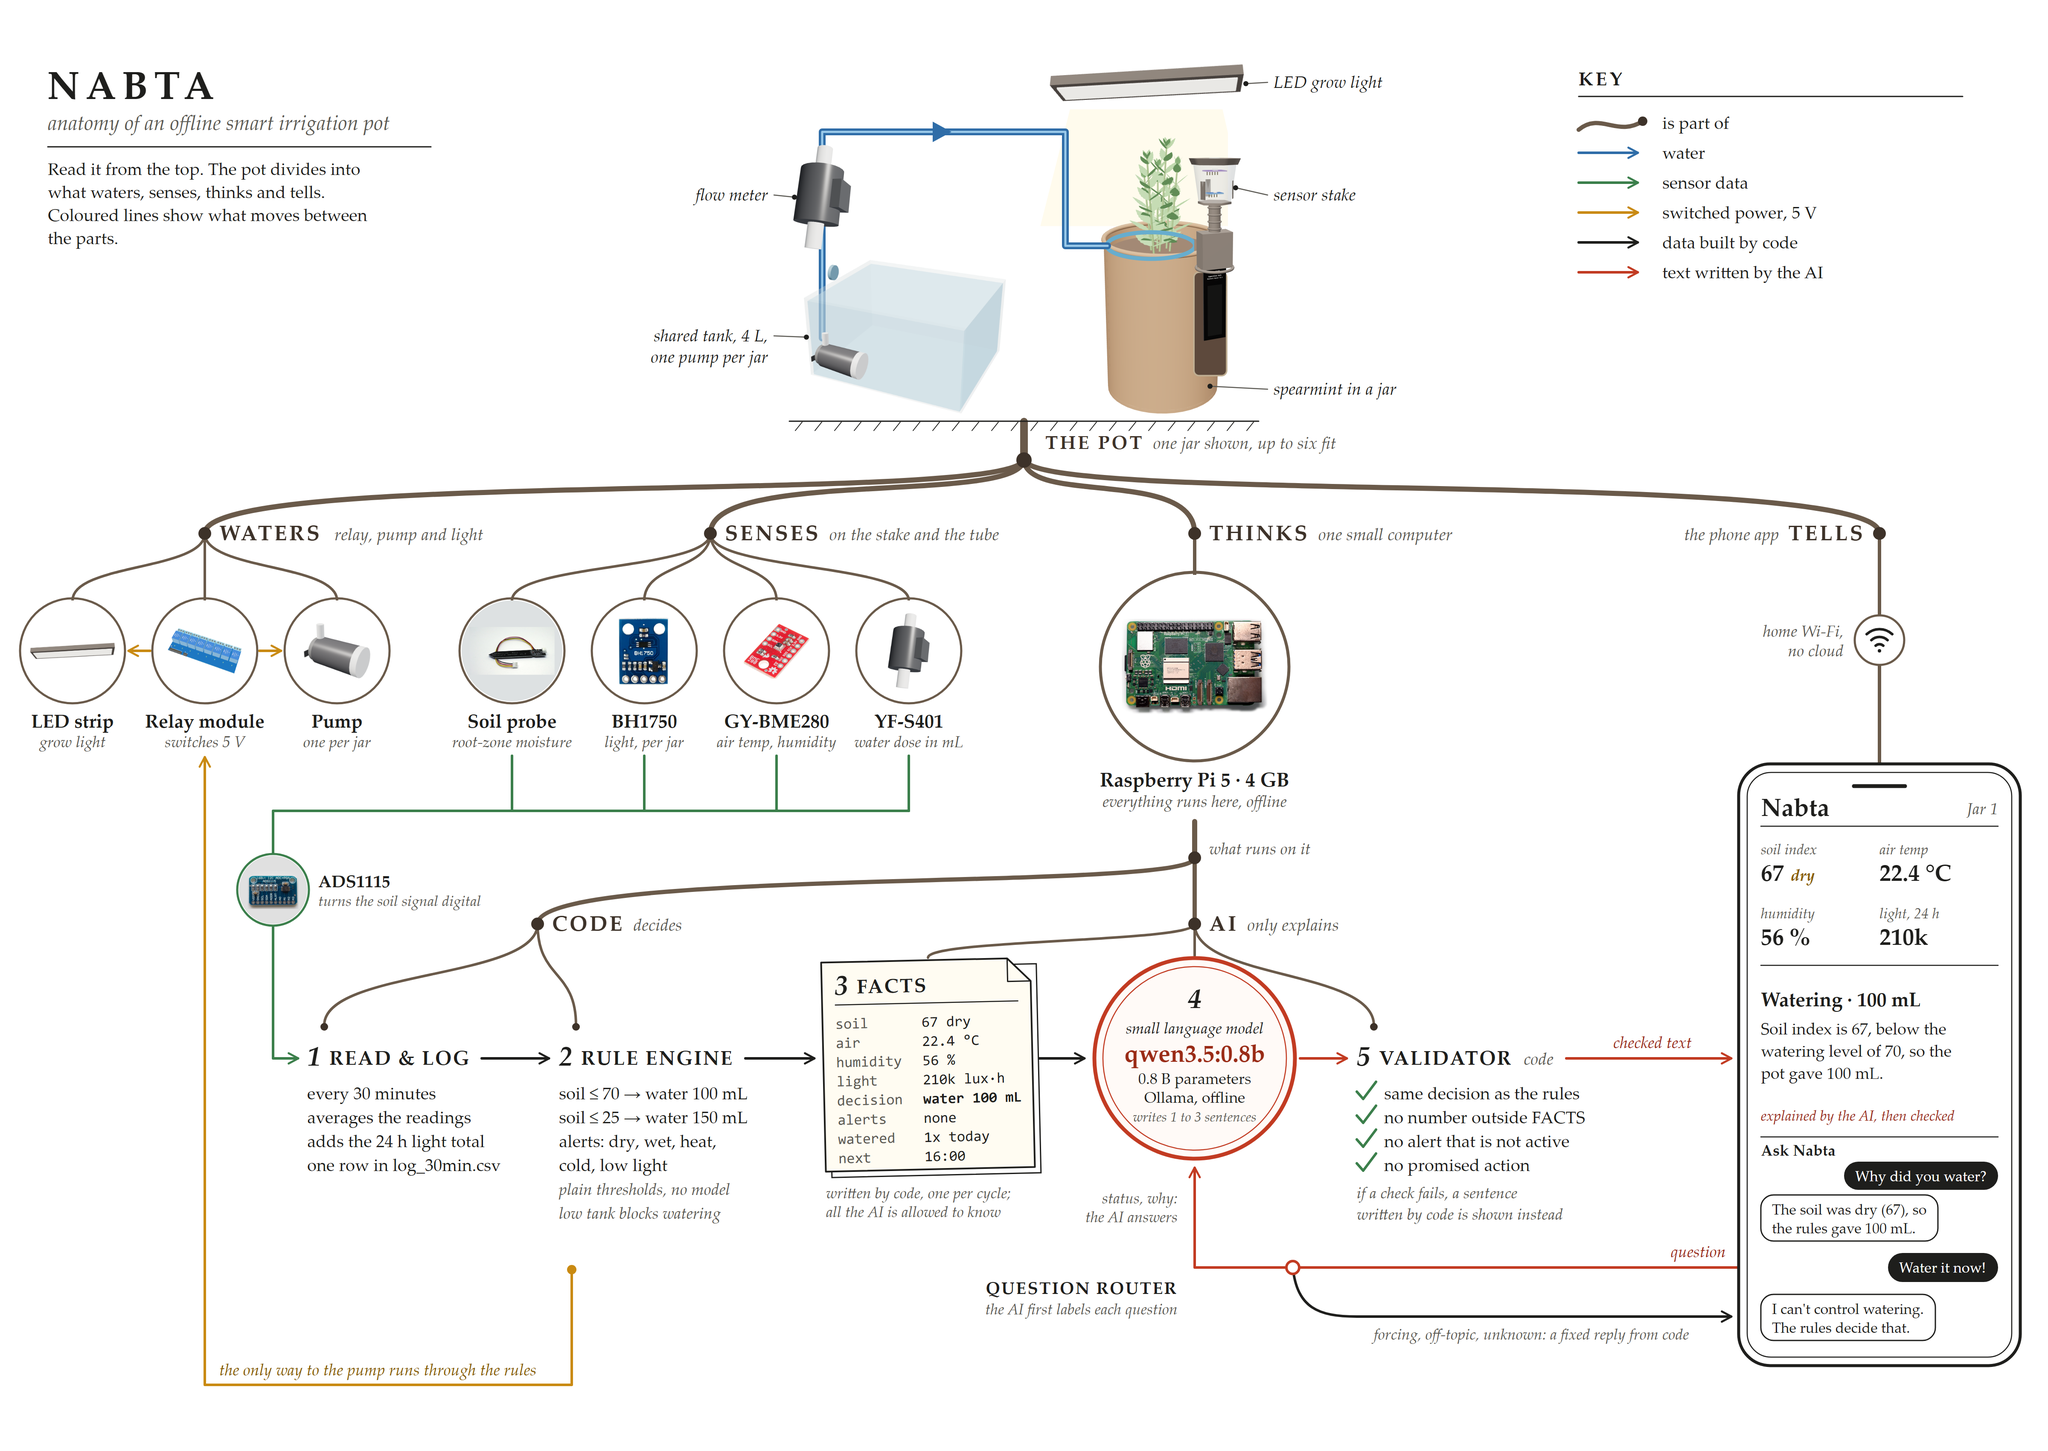
\includegraphics[width=\textwidth]{fig1_system_overview.png}
  \caption{Anatomy of Nabta. The pot \emph{waters}, \emph{senses}, \emph{thinks} and \emph{tells}. Every 30 minutes the Raspberry Pi~5 reads and logs the sensors (1); a rule engine with plain thresholds decides whether to water (2); code writes a FACTS card (3), the only input the local model \texttt{qwen3.5:0.8b} may use to explain the decision in 1--3 sentences (4); a validator checks the text against the rules and FACTS and replaces it with a code-written sentence on failure (5). A question router sends forcing, off-topic and unknown questions to fixed replies. The pump can only be reached through the rules; nothing runs in the cloud.}
  \label{fig:system}
\end{figure*}

\subsection{Waters}
% LED strip, 5 V relay, one pump per jar, shared 4 L tank, YF-S401 flow meter (mL per dose).
\todo{}
\subsection{Senses}
% Soil probe via ADS1115, BH1750, GY-BME280; 30-min averages, 24 h light total.
\todo{}
\subsection{Thinks: rules decide, the AI explains}
% Steps 1--5 of Fig.~\ref{fig:system}; validator checks; question router.
\todo{}
\begin{lstlisting}[caption={A FACTS card, built by code each cycle.},label=lst:facts]
soil 67 dry | air 22.4 C | humidity 56 % | light 210k lux.h
decision water 100 mL | alerts none | watered 1x today | next 16:00
\end{lstlisting}
\subsection{Tells}
% Phone app over home Wi-Fi, no cloud; checked explanation; Ask Nabta.
\todo{}
% Table 1: bill of materials \todo{prices}

%==================================================================
\section{Experimental Design}\label{sec:design}
\subsection{Research questions and hypotheses}
% Main RQ, RQ1--RQ3, H1--H3 (docs/methods.md section 0).
\todo{}

\subsection{Controllers compared}
\begin{table}[t]\centering\small
\caption{Controllers. All receive the same live context every 30 min. Only rules reach the pump.}
\label{tab:controllers}
\begin{tabular}{@{}llll@{}}\toprule
ID & Controller & Runs on & Evaluated as\\\midrule
C1 & Single threshold & Pi & real Pot B; replay\\
C2 & Multi-rule (reference) & Pi & real Pot A; replay\\
C3 & Qwen3.5 0.8B & Pi, offline & shadow; replay\\
C4 & ChatGPT & cloud API & shadow on logs; replay\\
\bottomrule\end{tabular}\end{table}
% C3/C4 asked for the decision JSON {action, ml, reason}; ChatGPT used only offline on logged data.
\todo{}

\subsection{Frozen LLM settings}
\begin{table}[t]\centering\small
\caption{Decoding settings, identical for C3 and C4.}
\label{tab:params}
\begin{tabular}{@{}ll@{}}\toprule
Parameter & Value\\\midrule
Temperature & 0\\ Top-$p$ & 1\\ Max tokens & 200\\ Seed & 42\\ Context window & 4096\\ Output & JSON only, no retries\\
\bottomrule\end{tabular}\end{table}

\subsection{Plants and setup}
Spearmint (\emph{Mentha spicata}) needs frequent watering~\cite{NSW}, grows best at 15--25\,$^\circ$C~\cite{OMAFRA} and survives 4--36\,$^\circ$C~\cite{ISWS}; its growth falls below field capacity~\cite{FUM}, and under sustained deficit fresh yield drops while water-use efficiency rises~\cite{OKW11}. Extension guidance waters water-sensitive crops after about 30\% of available water is depleted~\cite{VT}, which sets our watering threshold \todo{match the final threshold: 60 (kit) or 70 (diagram)}.
\todo{two jars, same batch, swap every 4 days, [14] days, daily weight / wilting / photo}
\subsection{Evaluation modes}
% Real pots (C1, C2); shadow mode (all); closed-loop replay (all), validated against real pots.
\todo{}
\subsection{Hard cases and offline test}
\todo{40 near-threshold cases x 3 repeats; one planned network cut}

%==================================================================
\section{Metrics}\label{sec:metrics}
% Table 4: RQ1 precision, RQ2 reliability, RQ3 cost (docs/metrics.md). Optional: validator pass rate, router accuracy.
\todo{}

%==================================================================
\section{Results}\label{sec:results}
% Only numbers from experiment/metrics.py on real logs.
\subsection{Irrigation precision (RQ1)}
% Fig. 2 moisture traces; Table 5; sim-vs-real error. Verdict on H1.
\todo{}
\subsection{Decision reliability (RQ2)}
% Table 6 routine vs. hard cases; error analysis. Verdict on H2.
\todo{}
\subsection{Operational cost (RQ3)}
% Fig. 3 kappa vs. latency vs. cost; offline cut. Verdict on H3.
\todo{}
\subsection{Explanation layer (optional)}
\todo{validator pass rate, fallback rate, router accuracy}

%==================================================================
\section{Discussion}\label{sec:discussion}
% Decide or only explain? Cost/privacy vs. accuracy.
\todo{}
\subsection*{Limitations}
\todo{one plant per real arm; 14 days; one species; LLMs in shadow and simulation; C2 is controller and reference; simulator calibration; ChatGPT after the fact}

%==================================================================
\section{Conclusion and Future Work}\label{sec:conclusion}
\todo{answer to the main RQ; more jars, longer runs, validated model under the gate, RAG}

\section*{Acknowledgements}
\todo{}

\bibliographystyle{plain}
\bibliography{refs}

% Appendix (if allowed): A system prompt; B validator rules and router labels; C hard-case list.
\end{document}
